\documentclass[journal,12pt,twocolumn]{IEEEtran}

\usepackage{setspace}
\usepackage{gensymb}
\singlespacing
\usepackage[cmex10]{amsmath}

\usepackage{amsthm}

\usepackage{mathrsfs}
\usepackage{txfonts}
\usepackage{stfloats}
\usepackage{bm}
\usepackage{cite}
\usepackage{cases}
\usepackage{subfig}
\usepackage{paralist}
\usepackage{longtable}
\usepackage{multirow}

\usepackage{enumitem}
\usepackage{mathtools}
\usepackage{steinmetz}
\usepackage{tikz}
\usepackage{circuitikz}
\usepackage{verbatim}
\usepackage{tfrupee}
\usepackage[breaklinks=true]{hyperref}
\usepackage{graphicx}
\usepackage{tkz-euclide}

\usetikzlibrary{calc,math}
\usepackage{listings}
    \usepackage{color}                                            %%
    \usepackage{array}                                            %%
    \usepackage{longtable}                                        %%
    \usepackage{calc}                                             %%
    \usepackage{multirow}                                         %%
    \usepackage{hhline}                                           %%
    \usepackage{ifthen}                                           %%
    \usepackage{lscape}     
\usepackage{multicol}
\usepackage{chngcntr}


\usetikzlibrary{calc,math}
\usepackage{listings}
    \usepackage{color}                                            %%
    \usepackage{array}                                            %%
    \usepackage{longtable}                                        %%
    \usepackage{calc}                                             %%
    \usepackage{multirow}                                         %%
    \usepackage{hhline}                                           %%
    \usepackage{ifthen}                                           %%
    \usepackage{lscape}     
\usepackage{multicol}
\usepackage{chngcntr}

\DeclareMathOperator*{\Res}{Res}

\renewcommand\thesection{\arabic{section}}
\renewcommand\thesubsection{\thesection.\arabic{subsection}}
\renewcommand\thesubsubsection{\thesubsection.\arabic{subsubsection}}

\renewcommand\thesectiondis{\arabic{section}}
\renewcommand\thesubsectiondis{\thesectiondis.\arabic{subsection}}
\renewcommand\thesubsubsectiondis{\thesubsectiondis.\arabic{subsubsection}}


\hyphenation{op-tical net-works semi-conduc-tor}
\def\inputGnumericTable{}                                 %%

\lstset{
%language=C,
frame=single, 
breaklines=true,
columns=fullflexible
}
\begin{document}

\newcommand{\BEQA}{\begin{eqnarray}}
\newcommand{\EEQA}{\end{eqnarray}}
\newcommand{\define}{\stackrel{\triangle}{=}}
\bibliographystyle{IEEEtran}
\raggedbottom
\setlength{\parindent}{0pt}
\providecommand{\mbf}{\mathbf}
\providecommand{\pr}[1]{\ensuremath{\Pr\left(#1\right)}}
\providecommand{\qfunc}[1]{\ensuremath{Q\left(#1\right)}}
\providecommand{\sbrak}[1]{\ensuremath{{}\left[#1\right]}}
\providecommand{\lsbrak}[1]{\ensuremath{{}\left[#1\right.}}
\providecommand{\rsbrak}[1]{\ensuremath{{}\left.#1\right]}}
\providecommand{\brak}[1]{\ensuremath{\left(#1\right)}}
\providecommand{\lbrak}[1]{\ensuremath{\left(#1\right.}}
\providecommand{\rbrak}[1]{\ensuremath{\left.#1\right)}}
\providecommand{\cbrak}[1]{\ensuremath{\left\{#1\right\}}}
\providecommand{\lcbrak}[1]{\ensuremath{\left\{#1\right.}}
\providecommand{\rcbrak}[1]{\ensuremath{\left.#1\right\}}}
\theoremstyle{remark}
\newtheorem{rem}{Remark}
\newcommand{\sgn}{\mathop{\mathrm{sgn}}}
\providecommand{\abs}[1]{\vert#1\vert}
\providecommand{\res}[1]{\Res\displaylimits_{#1}} 
\providecommand{\norm}[1]{\lVert#1\rVert}
%\providecommand{\norm}[1]{\lVert#1\rVert}
\providecommand{\mtx}[1]{\mathbf{#1}}
\providecommand{\mean}[1]{E[ #1 ]}
\providecommand{\fourier}{\overset{\mathcal{F}}{ \rightleftharpoons}}
%\providecommand{\hilbert}{\overset{\mathcal{H}}{ \rightleftharpoons}}
\providecommand{\system}{\overset{\mathcal{H}}{ \longleftrightarrow}}
	%\newcommand{\solution}[2]{\textbf{Solution:}{#1}}
\newcommand{\solution}{\noindent \textbf{Solution: }}
\newcommand{\cosec}{\,\text{cosec}\,}
\providecommand{\dec}[2]{\ensuremath{\overset{#1}{\underset{#2}{\gtrless}}}}
\newcommand{\myvec}[1]{\ensuremath{\begin{pmatrix}#1\end{pmatrix}}}
\newcommand{\mydet}[1]{\ensuremath{\begin{vmatrix}#1\end{vmatrix}}}
\numberwithin{equation}{subsection}
\makeatletter
\@addtoreset{figure}{problem}
\makeatother
\let\StandardTheFigure\thefigure
\let\vec\mathbf
\renewcommand{\thefigure}{\theproblem}
\def\putbox#1#2#3{\makebox[0in][l]{\makebox[#1][l]{}\raisebox{\baselineskip}[0in][0in]{\raisebox{#2}[0in][0in]{#3}}}}
     \def\rightbox#1{\makebox[0in][r]{#1}}
     \def\centbox#1{\makebox[0in]{#1}}
     \def\topbox#1{\raisebox{-\baselineskip}[0in][0in]{#1}}
     \def\midbox#1{\raisebox{-0.5\baselineskip}[0in][0in]{#1}}
\vspace{3cm}
\title{AI1103-Assignment 2}
\author{Name: Avula Mohana Durga Dinesh Reddy , Roll Number: CS20BTECH11005}
\maketitle
\newpage
\bigskip
\renewcommand{\thefigure}{\theenumi}
\renewcommand{\thetable}{\theenumi}
Download all python codes from 
\begin{lstlisting}
https://github.com/DineshAvulaMohanaDurga/AI1103/blob/main/assignment_2/codes/ai1103_assignment1.py
\end{lstlisting}
%
and latex codes from 
%
\begin{lstlisting}
https://github.com/DineshAvulaMohanaDurga/AI1103/blob/main/assignment_2/main.tex
\end{lstlisting}
\section{Question}
(GATE-1999 problem-1.31) The joint probability density function of the random variables X, Y and Z is
\begin{align}
    f(x,y,z)&=8xyz, 0<x,y,z<1 \nonumber \\
    &=0 \text{ otherwise}
\end{align}
Then P($X<Y<Z$) is\\
\begin{inparaenum}[(A)]
\item $\frac{1}{8}$ \hspace{1cm}
\item $\frac{1}{3}$ \hspace{1cm}
\item $\frac{1}{6}$ \hspace{1cm}
\item $\frac{3}{8}$ \hspace{1cm}
\end{inparaenum}
\section{Answer}
Given joint probability density function j.d.f 
\begin{align}
    f(x,y,z)&=8xyz, 0<x,y,z<1 \nonumber \\
    &=0 \text{ otherwise}
\end{align}
we know that probability distribution function 
\begin{align}
    f(x)&=\int _{-\infty}^{\infty}\int _{-\infty}^{\infty} \text{f(x,y,z) dy dz} 
\end{align}
    \text{When 0$<$x$<$1}
\begin{align}
    & =\int _{-\infty}^{\infty}\brak{\int _{-\infty}^{0}\text{0 dy} + \int _0 ^1 \text{8xyz dy} +\int _{1}^{\infty}\text{0 dy}} dz \\
    &=\int _{-\infty}^{\infty}\brak{0 + 8xz \int _{0}^{1} \text{y dy} + 0}dz \nonumber
\end{align}
\begin{align}
    &=\int _{-\infty}^{\infty}\brak{8xz \times \frac{1}{2}} dz \nonumber \\
    &=4x\int _{-\infty}^{\infty}\text{z dz} \nonumber\\
    &=2x\\
\text{When x$<$0 or x$>1$:-} \nonumber \\
    &= \int _{-\infty}^{\infty}\int _{-\infty}^{\infty} \text{0 dy dz}\\
    &=0\\
\end{align}
\begin{align}
    \Rightarrow f(x)&=2x &\text{0$<x<1$} \nonumber\\
    &=0 &x<0\text{ or }x>1
\end{align}
similarly 
\begin{align}
f(y)&=2y  &\text{0$<y<1$} \nonumber\\
    &=0 &y<0\text{ or }y>1
\end{align}
and 
\begin{align}
f(z)&=2z  &\text{0$<z<1$} \nonumber\\
    &=0 &z<0\text{ or }z>1
\end{align}
assuming $0<x,y,z<1$ as the pdf is 0 
\begin{align}
\pr{x<y}&=\int _{-\infty}^y f\brak{x} dx\\
&=\int _{-\infty} ^0 \text{ 0 dx} +\int _0^y \text{2x dx}\\
&=y^2
\end{align}
\begin{align}
\pr{x<y<z}&=\int_{-\infty}^{\infty} f\brak{z}\brak{\int _{-\infty}^z \pr{x<y}\times f\brak{y}dy}dz\\
&=\int_{-\infty}^{\infty}f\brak{z}\brak{\int_{-\infty}^0 \text{0 dy }+ \int _0^z 2y^3dy}dz\nonumber\\
&=\int_{-\infty}^{\infty}f\brak{z}\frac{z^4}{2}dz\nonumber\\
&=\int_{-\infty}^{0}\text{ 0 dz}+\int_{0}^{1}z^5\text{ dz} +\int_{1}^{\infty}\text{ 0 dz}\nonumber\\
&=\frac{1}{6}
\end{align}
$\therefore$ The value of $\pr{X<Y<Z}$ is $\frac{1}{6}$ \\
$\therefore$ option C is correct
\begin{figure}[h!]
    \centering
    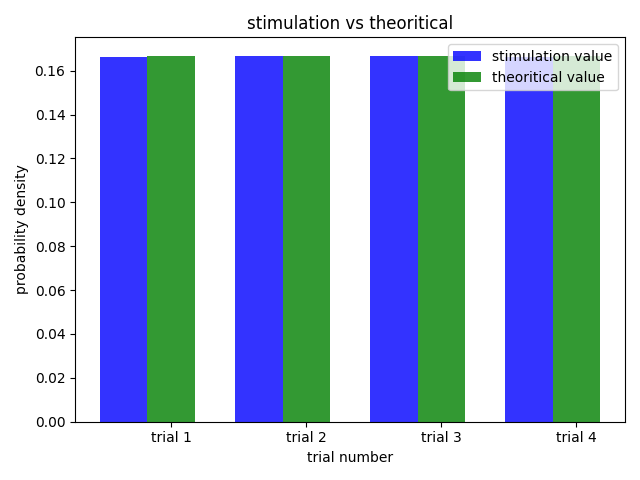
\includegraphics{figure_1.png}
    \caption{Simulation vs Theoritical}
    \label{fig:my_label}
\end{figure}
\end{document}
